\documentclass{article}
\usepackage{graphicx}
\usepackage{float} 
\usepackage{changepage}
\usepackage{tikz-among-us} % Mainly for memes
\usepackage{xcolor}
\usepackage{framed}
\usepackage{amssymb}
\usepackage{amsmath}
\usepackage{cancel} % Allows trikethrough in equations
\usepackage{enumitem} % This package allows more customization of lists
\usepackage[margin=1in]{geometry}  % Adjust the margin size as needed
\usepackage{tabularx}
\newenvironment{amatrix}[1]{%
  \left(\begin{array}{@{}*{#1}{c}|c@{}}
}{%
  \end{array}\right)
}

% environment derived from framed.sty: see leftbar environment definition
\definecolor{formalshade}{rgb}{0.95,1,0.95}
\definecolor{darkblue}{rgb}{0.0,0.5,0.5}     % dark green for the left bar

\newenvironment{formal}{%
  \def\FrameCommand{%
    \hspace{1pt}%
    {\color{darkblue}\vrule width 2pt}%
    {\color{formalshade}\vrule width 4pt}%
    \colorbox{formalshade}%
  }%
  \MakeFramed{\advance\hsize-\width\FrameRestore}%
  \noindent\hspace{-4.55pt}% disable indenting first paragraph
  \begin{adjustwidth}{}{7pt}%
  \vspace{2pt}\vspace{2pt}%
}
{%
  \vspace{2pt}\end{adjustwidth}\endMakeFramed%
}

\title{Title}
\author{
  Christopher Erickson\\
}
\date{\today}

\begin{document}

\maketitle
\section*{Glossary}
\begin{table}[h!]
\centering
\begin{tabularx}{\textwidth}{|l|X|}
\hline
\textbf{dim} & Dimension of the cell i.e. 1-d, 2d, 3d \\ \hline
\textbf{spacedim} & Dimension of the problem space, i.e. what the cell resides in \\ \hline
\textbf{celltype} & Type of mapping, linear or quadratic. \\ \hline
\end{tabularx}
\caption{Description of cell properties}
\end{table}
\section*{Data Format}
% \begin{formal}
% \end{formal}

\section*{Constants}
\begin{table}[h!]
\centering
\begin{tabularx}{\textwidth}{|l|X|}
\hline
\textbf{dim} & Dimension of the cell i.e. 1-d, 2d, 3d \\ \hline
\end{tabularx}
\caption{Description of cell properties}
\end{table}
\section*{Functions}
\subsection{UpdateFlags(const UpdateFlags f1, const UpdateFlags f2)}

\section{Configuration Header \texttt{config.h}}

This header defines fundamental types, constants, and helper functions used throughout the \texttt{dromon} library.

\subsection{Namespace Macros}

\begin{description}
  \item[\texttt{\#define DROMON\_NAMESPACE\_OPEN}] Expands to \texttt{namespace dromon \{}.
  \item[\texttt{\#define DROMON\_NAMESPACE\_CLOSE}] Closes the namespace.
\end{description}

\subsection{Polynomial Degree Macros}
These macros define polynomial orders used in the basis functions:
\begin{itemize}
  \item \texttt{LINEARP}: 0
  \item \texttt{QUADRATICP}: 1
  \item \texttt{CUBICP}: 2
\end{itemize}

\subsection{Enumerations}

\subsubsection*{DoFDirection}
\begin{verbatim}
enum DoFDirection { u_dir, v_dir, w_dir };
\end{verbatim}
Represents the direction of the degree of freedom.

\subsubsection*{CurrentType}
\begin{verbatim}
enum CurrentType { Electric, Magnetic, Nothing };
\end{verbatim}
Indicates the type of current.

\subsubsection*{UpdateFlags}
\begin{verbatim}
enum UpdateFlags {
  update_default   = 0,
  output_active    = 0x000001,
  verbose_output   = 0x000040,
  suppress_comments= 0x000002
};
\end{verbatim}
Flags controlling output and verbosity. These can be combined with bitwise operators:
\[
f = output\_active \mid verbose\_output
\]

\subsubsection*{RegularityType}
\begin{verbatim}
enum RegularityType {
  SelfSingular,
  FaceSingular,
  EdgeSingular,
  PointSingular,
  FaceNearSingular,
  EdgeNearSingular,
  PointNearSingular,
  Regular
};
\end{verbatim}
Classifies singularity types encountered in geometries.

\subsubsection*{AdjacencyType}
\begin{verbatim}
enum AdjacencyType {
  Disjoint,
  Self,
  Face,
  Edge,
  Vertex
};
\end{verbatim}
Specifies how two cells are adjacent.

\subsection{Bitwise Operator Overloads}

\texttt{UpdateFlags} supports bitwise operators:
\begin{itemize}
  \item \texttt{operator|(UpdateFlags, UpdateFlags)}: bitwise OR
  \item \texttt{operator\&(UpdateFlags, UpdateFlags)}: bitwise AND
\end{itemize}

\subsection{GeometryInfo Template}
\begin{verbatim}
template <unsigned int dim,
          unsigned int spacedim,
          unsigned int surf_type>
struct GeometryInfo {
  static constexpr unsigned int nodes_per_cell;
  static constexpr unsigned int vertices_per_cell;
  static constexpr unsigned int faces_per_cell;
  static constexpr unsigned int vertices_per_face;
};
\end{verbatim}

This struct provides compile-time constants describing geometric properties.

\paragraph{Definition of \texttt{nodes\_per\_cell}:}
\[
\text{nodes\_per\_cell} =
\begin{cases}
(surf\_type + 2), & \text{if } dim = 1\\[6pt]
(surf\_type + 2)^2, & \text{if } dim = 2\\[6pt]
(surf\_type + 2)^3, & \text{if } dim = 3
\end{cases}
\]

\paragraph{Other Constants:}
\[
\text{vertices\_per\_cell} = 2^{dim}
\]
\[
\text{faces\_per\_cell} = 2 \times dim
\]
\[
\text{vertices\_per\_face} = 2^{dim}
\]

\subsection{Stream Operators}
The following overloads are provided for formatted output:
\begin{verbatim}
std::ostream& operator<<(std::ostream&, const DoFDirection&);
std::ostream& operator<<(std::ostream&, const CurrentType&);
\end{verbatim}
These allow printing enums as strings.

\subsection{Example}
\begin{verbatim}
DoFDirection dir = v_dir;
std::cout << dir; // Prints "v_dir"

UpdateFlags flags = output_active | verbose_output;
\end{verbatim}
\subsection{Constants Template}

\begin{verbatim}
template <class Real>
struct constants
{
  static constexpr Real PI = 3.1415926535897932...;
  static constexpr Real C0 = 299792458.;
  static constexpr Real EPS0 = 8.8541878128e-12;
  static constexpr Real MU0 = PI * 4.0e-7;
  static constexpr Real ROOT_EPS0MU0_ = 3.335640951073527...e-9;
  static constexpr std::complex<Real> complexj = {Real(0), Real(1)};
};
\end{verbatim}

This template defines physical and mathematical constants used in the library.

\paragraph{Members:}
\begin{description}
  \item[\texttt{PI}] The mathematical constant $\pi$ to very high precision.
  \[
  \pi = 3.14159265358979323846\ldots
  \]
  \item[\texttt{C0}] The speed of light in vacuum:
  \[
  c_0 = 299,792,458 \text{ m/s}
  \]
  \item[\texttt{EPS0}] The vacuum permittivity:
  \[
  \varepsilon_0 = 8.8541878128 \times 10^{-12}\text{ F/m}
  \]
  \item[\texttt{MU0}] The vacuum permeability:
  \[
  \mu_0 = 4\pi \times 10^{-7}\text{ H/m}
  \]
  \item[\texttt{ROOT\_EPS0MU0\_}]
  \[
  \sqrt{\varepsilon_0 \mu_0} \approx 3.335640951073527 \times 10^{-9}
  \]
  This value frequently arises in electromagnetic formulations.
  \item[\texttt{complexj}]
  The imaginary unit:
  \[
  j = 0 + i
  \]
  stored as \texttt{std::complex<Real>\{0,1\}}.
\end{description}

\paragraph{Usage Example:}
\begin{verbatim}
Real pi = constants<Real>::PI;
std::complex<Real> j = constants<Real>::complexj;
Real eta = sqrt(constants<Real>::MU0 / constants<Real>::EPS0);
\end{verbatim}
\section{Class Template \texttt{DataOut}}

The \texttt{DataOut} class template handles exporting mesh and degrees-of-freedom data to VTK and auxiliary files.

\subsection*{Template Parameters}
\begin{description}
  \item[\texttt{dim}] Topological dimension of the cells (1, 2, or 3).
  \item[\texttt{spacedim}] Dimension of the embedding space.
  \item[\texttt{celltype}] Integer code specifying the type/order of the cell.
  \item[\texttt{CoefficientType}] Type for degrees of freedom coefficients (default: \texttt{std::complex<double>}).
  \item[\texttt{Real}] Floating point type (default: \texttt{double}).
\end{description}

\subsection*{Public Interface}

\begin{itemize}
  \item \texttt{DataOut()}
  \item \texttt{DataOut(Mesh*, std::string file\_path, UpdateFlags)}
  \item \texttt{DataOut(Mesh*, DoFHandler*, std::string file\_path, UpdateFlags)}
  \item \texttt{void attach\_mesh(Mesh*)}
  \item \texttt{void attach\_dof\_handler(DoFHandler*)}
  \item \texttt{void vtk\_out()}
  \item \texttt{void add\_cell\_data(std::vector<double>\&, std::string name="default")}
  \item \texttt{void set\_flags(UpdateFlags)}
\end{itemize}

\subsection*{Description}

This class provides methods to:
\begin{enumerate}
  \item Attach a mesh and (optionally) a degrees-of-freedom handler.
  \item Store scalar cell data (and potentially node data).
  \item Export:
    \begin{itemize}
      \item VTK files (\texttt{.vtk}) for visualization.
      \item Plain text files (\texttt{.global.dat}) containing metadata.
    \end{itemize}
\end{enumerate}

\subsection*{File Output}
\paragraph{VTK File}
\begin{itemize}
  \item Includes:
    \begin{itemize}
      \item Grid points
      \item Cell connectivity
      \item Cell types (VTK codes depending on \texttt{dim} and \texttt{celltype})
      \item Scalar cell data (if added)
    \end{itemize}
\end{itemize}

\paragraph{Global Data File}
\begin{itemize}
  \item Outputs summary statistics.
  \item If \texttt{UpdateFlags::verbose\_output} or \texttt{UpdateFlags::output\_active} are set, lists DoFs.
\end{itemize}

\subsection*{Example Usage}

\begin{verbatim}
DataOut<2,2,1> data_out(mesh, "output/myfile", UpdateFlags::verbose_output);
data_out.add_cell_data(cell_scalars, "stress");
data_out.vtk_out();
\end{verbatim}

\subsection*{Note on VTK Cell Ordering}
Higher-order cells follow VTK conventions. For example, a 2D quadratic cell is ordered as:
\begin{figure}[H]
    \centering
    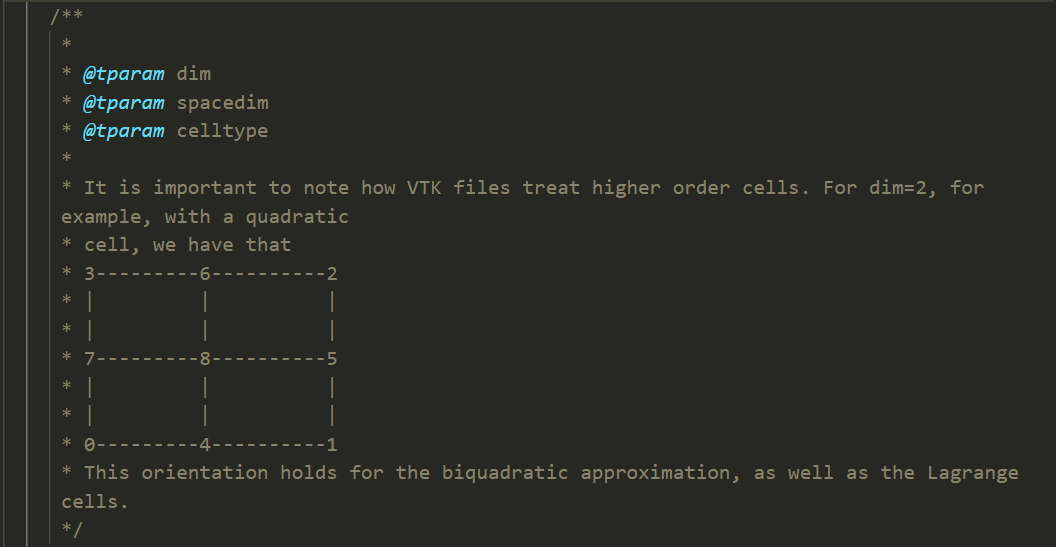
\includegraphics[width=0.75\linewidth]{P1.png}
    \caption{VTK Files}
    \label{}
\end{figure}

\subsection*{Dependencies}
This class depends on:
\begin{itemize}
  \item \texttt{Mesh}
  \item \texttt{DoFHandler}
  \item \texttt{DoFBase}
\end{itemize}
as well as \texttt{config.h}.

\end{document}